\documentclass[a4paper, article, oneside, norsk]{memoir} % Alternativt nynorsk

\usepackage{physics}
\setlength{\parindent}{0pt}

%% Tegnkoding
\usepackage[utf8]{inputenx} % Kildekode
\usepackage[T1]{fontenc}    % PDF

%% Fonter og typografi
\usepackage{lmodern}           % Latin Modern Roman
\usepackage[scaled]{beramono}  % Bera Mono (Bitstream Vera Sans Mono)
\renewcommand{\sfdefault}{phv} % Helvetica
\usepackage[final]{microtype}  % Forbedret typografi
\pretitle{\begin{center}\LARGE\sffamily\bfseries\boldmath}           % Tittel
\renewcommand{\abstractnamefont}{\sffamily\bfseries}                 % Sammendrag
\renewcommand*{\chaptitlefont}{\Large\bfseries\sffamily\raggedright} % Kapittel
\setsecheadstyle{\large\bfseries\sffamily\raggedright}               % Seksjon
\setsubsecheadstyle{\large\bfseries\sffamily\raggedright}            % Underseksjon
\setsubsubsecheadstyle{\normalsize\bfseries\sffamily\raggedright}    % Underunderseksjon
\setparaheadstyle{\normalsize\bfseries\sffamily\raggedright}         % Avsnitt
\setsubparaheadstyle{\normalsize\bfseries\sffamily\raggedright}      % Underavsnitt

%% Matematikk
\usepackage{amssymb}   % Ekstra symboler
\usepackage{amsthm}    % Teoremaktige omgivelser
\usepackage{thmtools}  % Teoremaktige omgivelser
\usepackage{mathtools} % Fonter og omgivelser for matematikk
\usepackage{mathrsfs}  % Scriptfont med \mathscr{}

%% Diverse
\usepackage{graphicx}  % Bilder
\usepackage{babel}     % Automatiske oversettelser
\usepackage{csquotes}  % Sitater
\usepackage{textcomp}  % Ekstra symboler
\usepackage{listings}  % Typesetting av kode
\lstset{basicstyle = \ttfamily, frame = tb}

%% Bibliografi
\usepackage{mathscinet}
\usepackage[backend    = biber,
            sortcites  = true,
            giveninits = true,
            doi        = false,
            isbn       = false,
            url        = false,
            style      = alphabetic]{biblatex}
\DeclareNameAlias{sortname}{family-given}
\DeclareNameAlias{default}{family-given}
\DeclareFieldFormat[article]{volume}{\bibstring{jourvol}\addnbspace#1}
\DeclareFieldFormat[article]{number}{\bibstring{number}\addnbspace#1}
\renewbibmacro*{volume+number+eid}
{
    \printfield{volume}
    \setunit{\addcomma\space}
    \printfield{number}
    \setunit{\addcomma\space}
    \printfield{eid}
}
%\addbibresource{<BIBLIOGRAFIFILNAVN>.bib}

%% Kryssreferanser
\usepackage{varioref}
\usepackage[pdfusetitle]{hyperref}
\urlstyle{sf}
\usepackage[nameinlink, noabbrev]{cleveref}
\crefname{chapter}{seksjon}{seksjoner}
\Crefname{chapter}{Seksjon}{Seksjoner}

%% Kompensasjon for lange ord i norsk
\pretolerance = 2000
\tolerance    = 6000
\hbadness     = 6000

%% Teoremaktige omgivelser
\declaretheorem[style = plain, numberwithin = chapter]{teorem}
\declaretheorem[style = plain,      sibling = teorem]{korollar}
\declaretheorem[style = plain,      sibling = teorem]{lemma}
\declaretheorem[style = plain,      sibling = teorem]{proposisjon}
\declaretheorem[style = definition, sibling = teorem]{definisjon}
\declaretheorem[style = definition, sibling = teorem]{eksempel}
\declaretheorem[style = remark,    numbered = no]{bemerkning}


%% Operatorer
\newcommand{\diff}{\mathop{}\!\mathrm{d}}
\DeclareMathOperator{\im}{im}
\DeclareMathOperator{\E}{E}
\DeclareMathOperator{\Var}{Var}
\DeclareMathOperator{\Cov}{Cov}

%% Nye kommandoer for mengder
\newcommand{\N}{\mathbb{N}}   % Naturlige tall
\newcommand{\Z}{\mathbb{Z}}   % Heltall
\newcommand{\Q}{\mathbb{Q}}   % Rasjonale tall
\newcommand{\R}{\mathbb{R}}   % Reelle tall
\newcommand{\C}{\mathbb{C}}   % Komplekse tall
\newcommand{\A}{\mathbb{A}}   % Affint rom
\renewcommand{\P}{\mathbb{P}} % Projektivt rom

%% Nye kommandoer for vektorer
\renewcommand{\a}{\mathbf{a}}
\renewcommand{\b}{\mathbf{b}}
\renewcommand{\c}{\mathbf{c}}
\renewcommand{\v}{\mathbf{v}}
\newcommand{\w}{\mathbf{w}}
\newcommand{\x}{\mathbf{x}}
\newcommand{\y}{\mathbf{y}}
\newcommand{\z}{\mathbf{z}}
\newcommand{\0}{\mathbf{0}}
\newcommand{\1}{\mathbf{1}}

%% For å vise kode 
\usepackage{listings}
\usepackage{xcolor}
 
\definecolor{codegreen}{rgb}{0,0.6,0}
\definecolor{codegray}{rgb}{0.5,0.5,0.5}
\definecolor{codepurple}{rgb}{0.58,0,0.82}
\definecolor{backcolour}{rgb}{0.95,0.95,0.92}
 
\lstdefinestyle{mystyle}{
    backgroundcolor=\color{backcolour},   
    commentstyle=\color{codegreen},
    keywordstyle=\color{magenta},
    numberstyle=\tiny\color{codegray},
    stringstyle=\color{codepurple},
    basicstyle=\ttfamily\footnotesize,
    breakatwhitespace=false,         
    breaklines=true,                 
    captionpos=b,                    
    keepspaces=true,                 
    numbers=left,                    
    numbersep=5pt,                  
    showspaces=false,                
    showstringspaces=false,
    showtabs=false,                  
    tabsize=2
}

\lstset{style=mystyle}

%% Diverse
\renewcommand{\qedsymbol}{\(\blacksquare\)}


\title{IN2010 - Oblig 3}
\author{Stian Østgaard \\ Thuan Tran \\
Embrik Thoresen}
\date{05.11.2021}

\begin{document}
\maketitle

\subsection*{Nyttig informasjon:}
Nedenfor er det informasjon knyttet til endring av prekode som er gjort, hvordan mappestrukturen vår ser ut og forklaring på hvordan man kjører koden.
\\ 
\subsubsection*{Endring av prekode:}
Vi har endret følgende kode fra 'oblig3runner.py'. Dette har vi gjort slik at når vi printer resultatet på deloppgave 1 til outputfilen som vi ønsker å skrive til, så printer vi filen til mappen 'outputs' som inneholder resultatene ved å kjøre en gitt algoritme på en inputfil fra mappen 'inputs'.

\begin{lstlisting} [language=Python]
def run_algs_part1(A, infilename):
    infilename = infilename.split("/")[1]
    for alg in ALGS1:
        countA = CountSwaps([CountCompares(x) for x in A])
        outfilename = "outputs/" + infilename + '_' + algname(alg) + '.out'
        outstr = '\n'.join(map(str, alg(countA)))
        with open(outfilename, 'w') as f:
            f.write(outstr)
\end{lstlisting}

Videre har vi også endret følgende kode fra 'oblig3runner.py'. Grunnen til dette er at vi igjen kjører algoritmene på en gitt inputfil fra mappen 'inputs' og skriver til en ny fil som befinner seg i mappen 'outputs'.

\begin{lstlisting} [language=Python]
def run_algs_part2(A, infilename):
    infilename = infilename.split("/")[1]
    outfilename = "outputs/" + infilename + '_results.csv'
    discarded = set()
   	...
\end{lstlisting}

Til slutt la vi til en konstruktør i 'countcompares.py' som man kan se på teksten nedenfor. Dette er ment for å overskride 'less than' slik at vi også kan teste 'less than or equal'.

\begin{lstlisting} [language=Python]
from functools import total_ordering

@total_ordering
class CountCompares:
    def __init__(self, elem):
        self.elem = elem
        self.compares = 0

    def reset(self):
        self.compares = 0

    def __eq__(self, other):
        return self.elem == other.elem

    def __lt__(self, other):
        self.compares += 1
        return self.elem < other.elem

    def __le__(self, other):
        self.compares += 1
        return self.elem <= other.elem

    def __repr__(self):
        return self.elem.__repr__()
\end{lstlisting}

\subsubsection*{Mappestrukturen vår:}
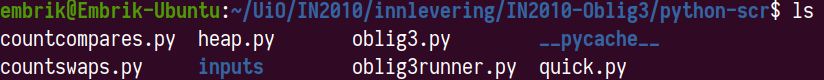
\includegraphics[scale=0.5]{mappe.png}
\\
Figur 1 - Mappestrukturen hvor filene er lagret inne i mappen 'python-scr'.


\subsubsection*{Kjøring av programmet:}

\includegraphics[scale=0.4]{runfile.png}
\\
Figur 2 - Hvordan kjøre programmene, der xxx står for ønsket inputfil fra mappen 'inputs'.

\subsection*{Deloppgave 1: Korrekthet}
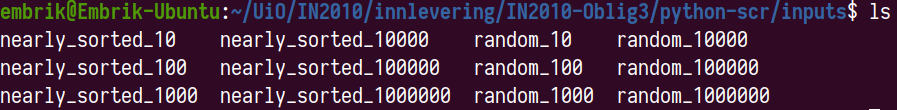
\includegraphics[scale=0.5]{IN2010oblig3_inputs.png}
\\
Figur 3 - Hvordan inputfilen vår ser ut. 
\\
\\
\\
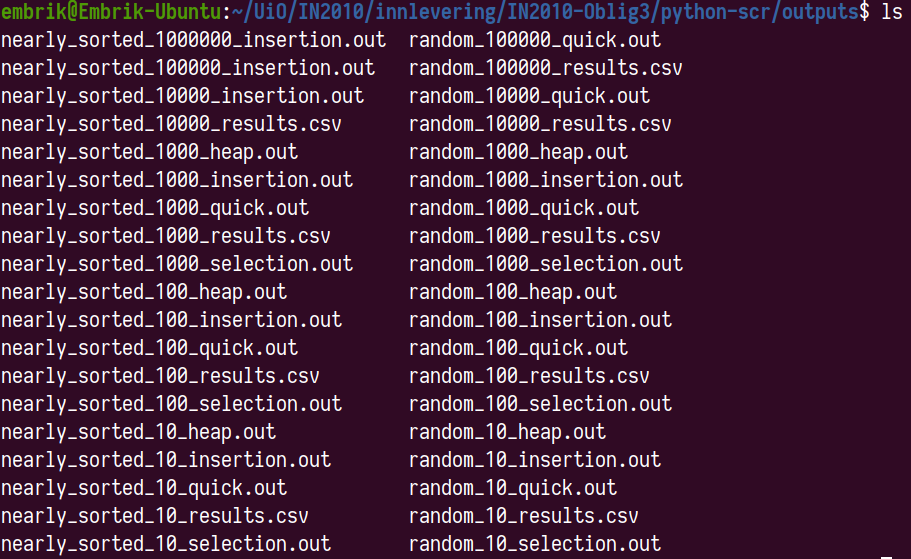
\includegraphics[scale=0.4]{IN2010oblig3_outputs.png}
\\
Figur 4 - Hvordan outputfilen vår ser ut.
\\
\\
Som man kan se på figur 4, har vi implementert insertion sort, selection sort, heapsort og quicksort. Vi har valgt å kun kjøre de algoritmene vi vet er raskest, basert på testing, på de største filene. For å teste at alle algoritmene gir rimelige svar har vi valgt å ...
\\
\subsection*{Deloppgave 2: Sammenligninger, bytter og tid}
Vi teller antall sammenligninger og bytter ved å bruke CountSwaps og CountCompares. For bytte to elementer i A kaller må man kalle på metoden A.swap(i,j) som bytter elementene A[i] og A[j] samtidig som man øker variablelen self.swaps med 1. Dermed vil self.swaps telle antall bytter i en algoritme. For å telle sammenligninger overskrider vi 'less than or equal' ($\leq$) og 'less than' ($<$) operasjonene til å øke variablelen self.comparisons med 1. Så self.comparisons teller antall sammenligninger i en algoritme. A eksisterer som en lokal instans i hvert algoritme-kall, dermed eksisterer disse telle-variablene lokalt.
\\
\\
Figurene under viser outputen når vi kjører 'random' og 'nearly sorted' med 1000 inputs. Til slutt printer vi ut den totale tiden målt i mikrosekunder. Det skal sies at vi fikk ulik svar når vi kjørte det på tre ulike PCer. Dette er grunnet timelimiten som er oppgitt i prekoden, hvor vi alle har forskjellige PCer.
\\
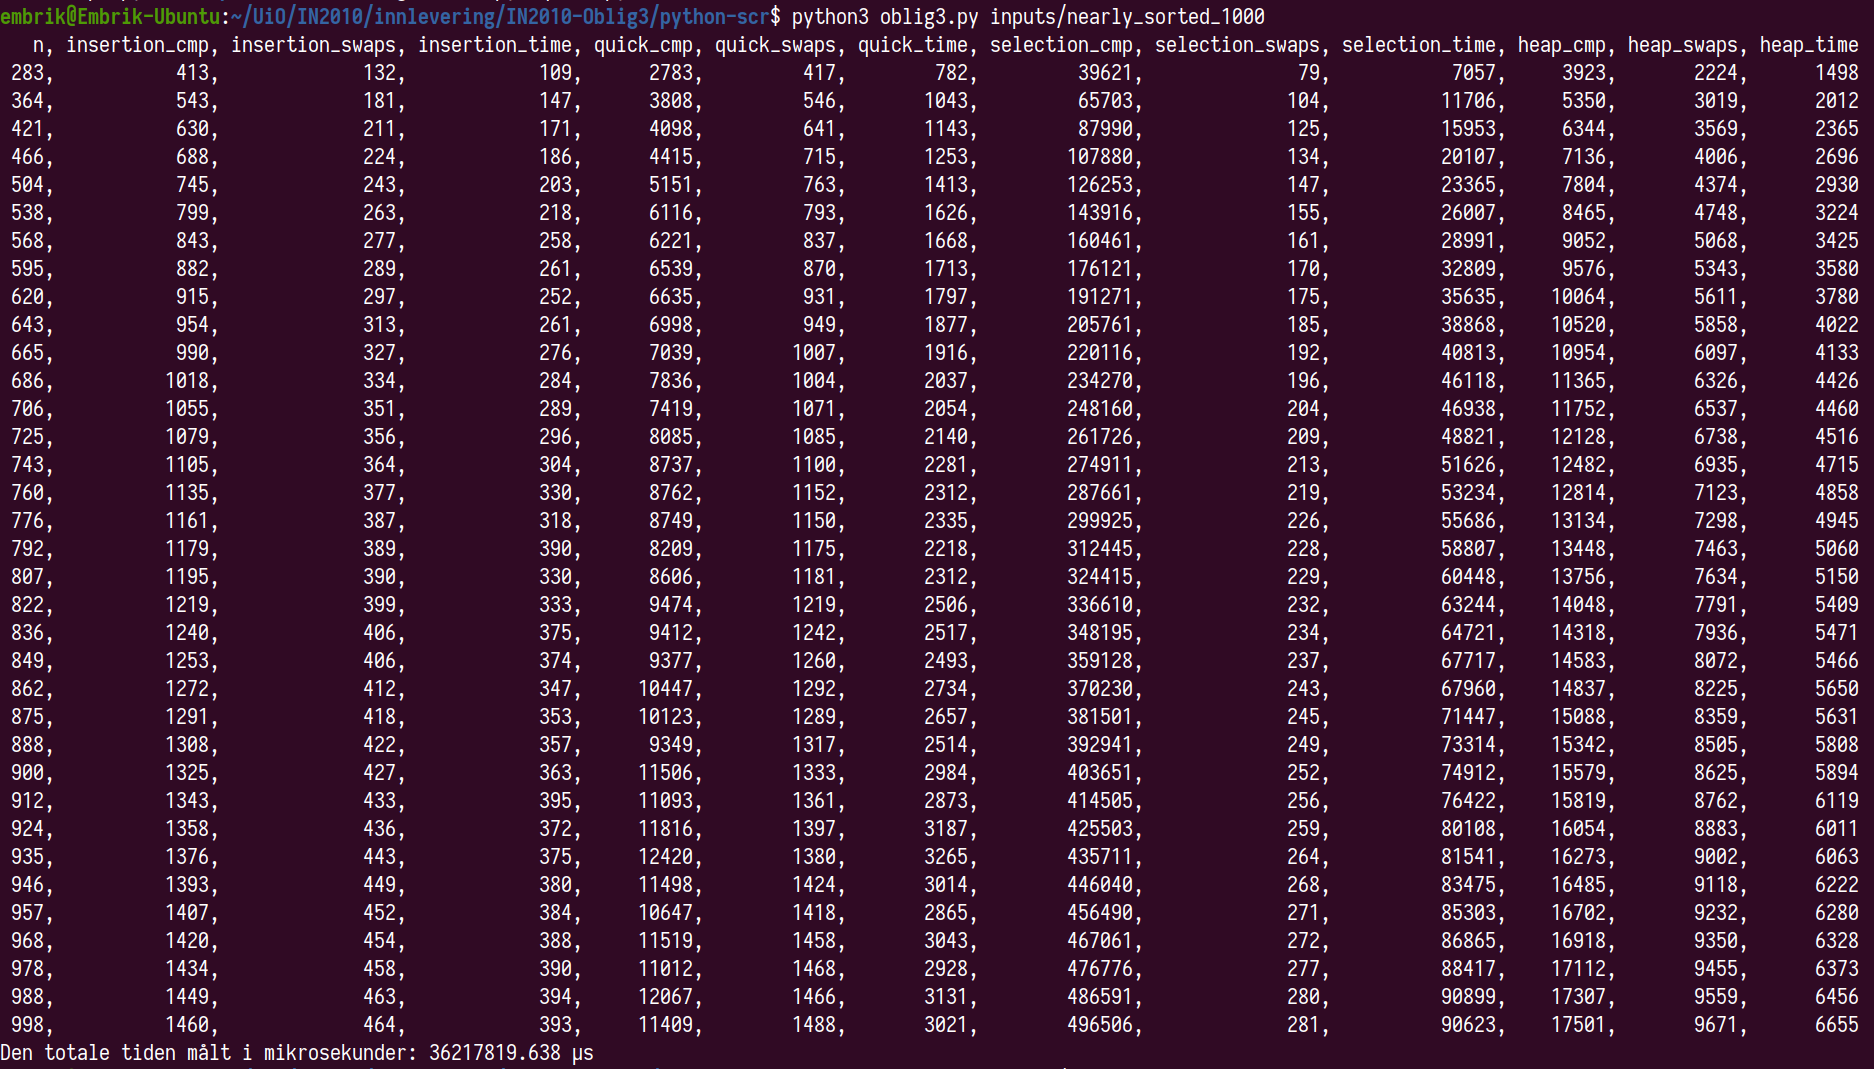
\includegraphics[scale=0.2]{IN2010oblig3_oppgave2a.png}
\\
Figur 5 - Outputen ved å kjøre filen 'nearly sorted' med 1000 inputs.
\\
\\
\\
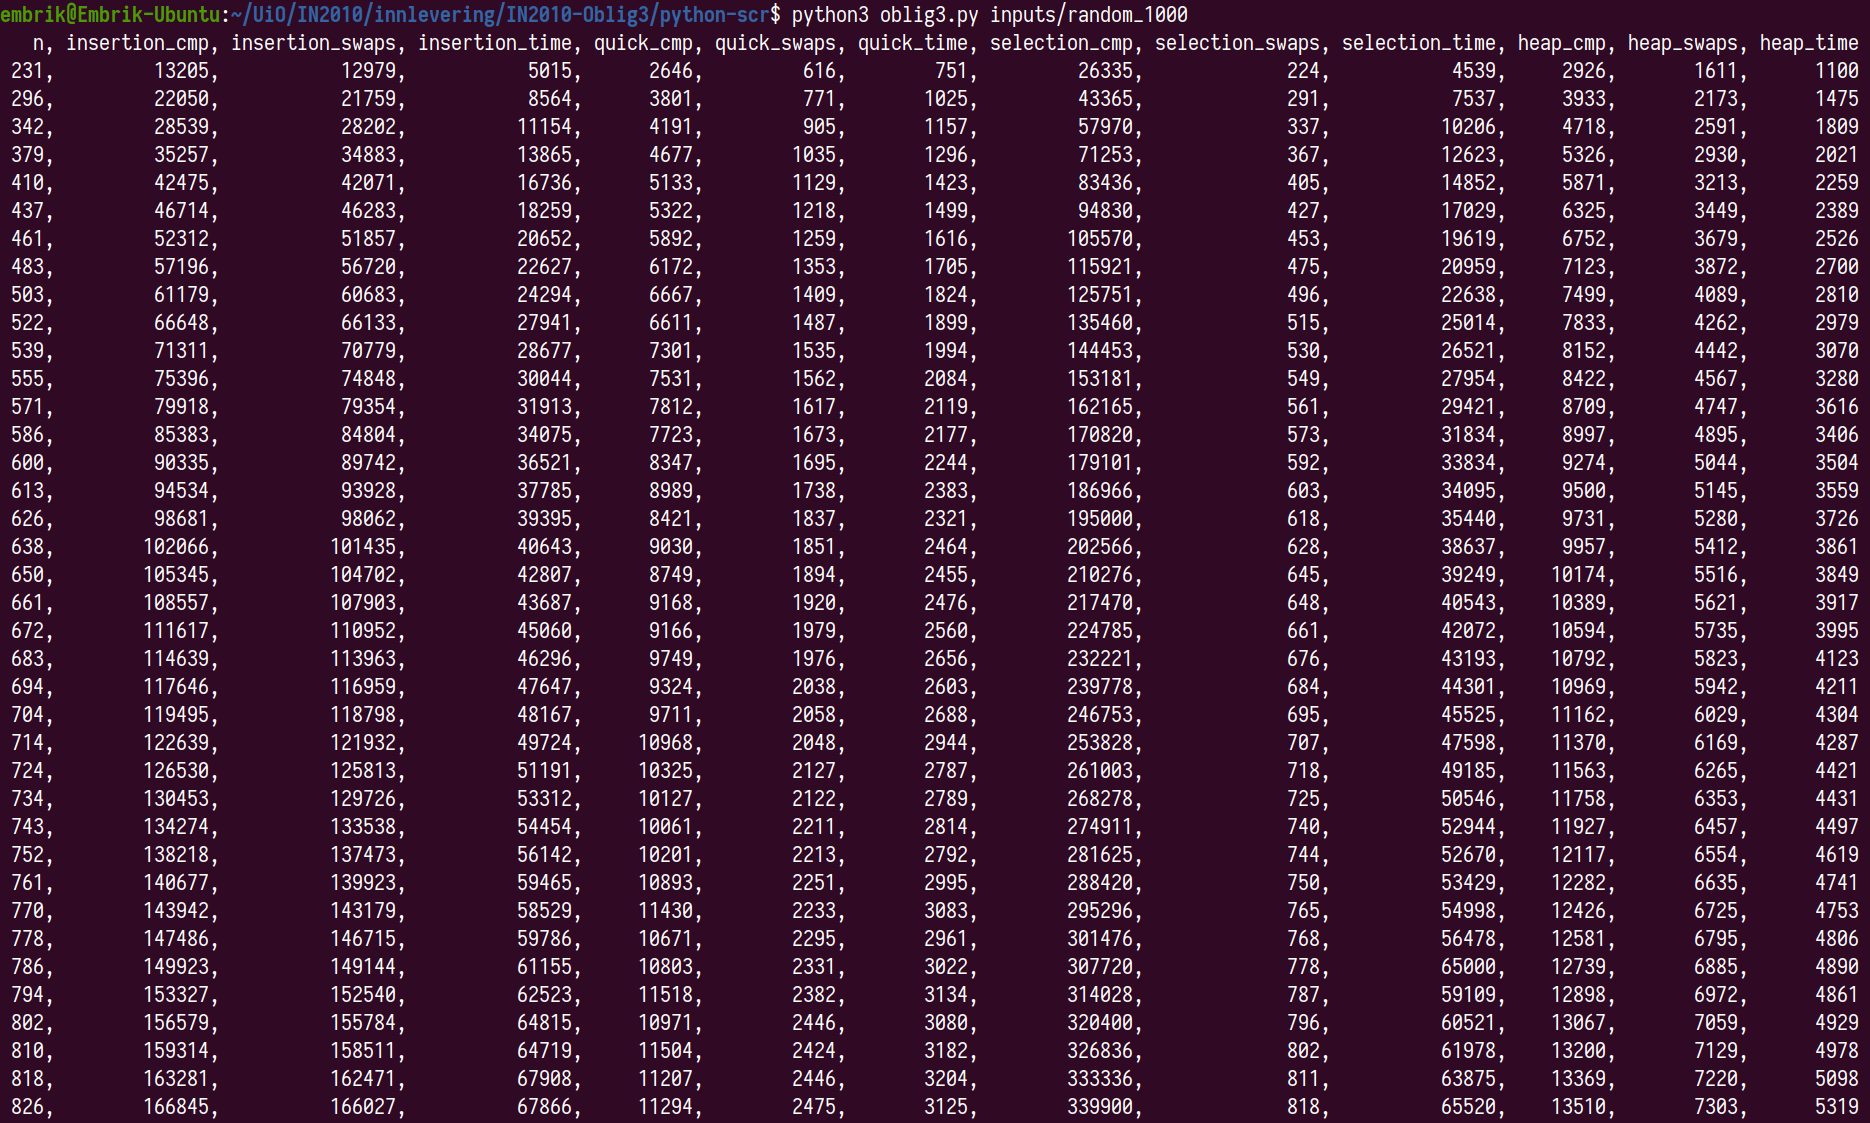
\includegraphics[scale=0.2]{IN2010oblig3_oppgave2c.png}
\\
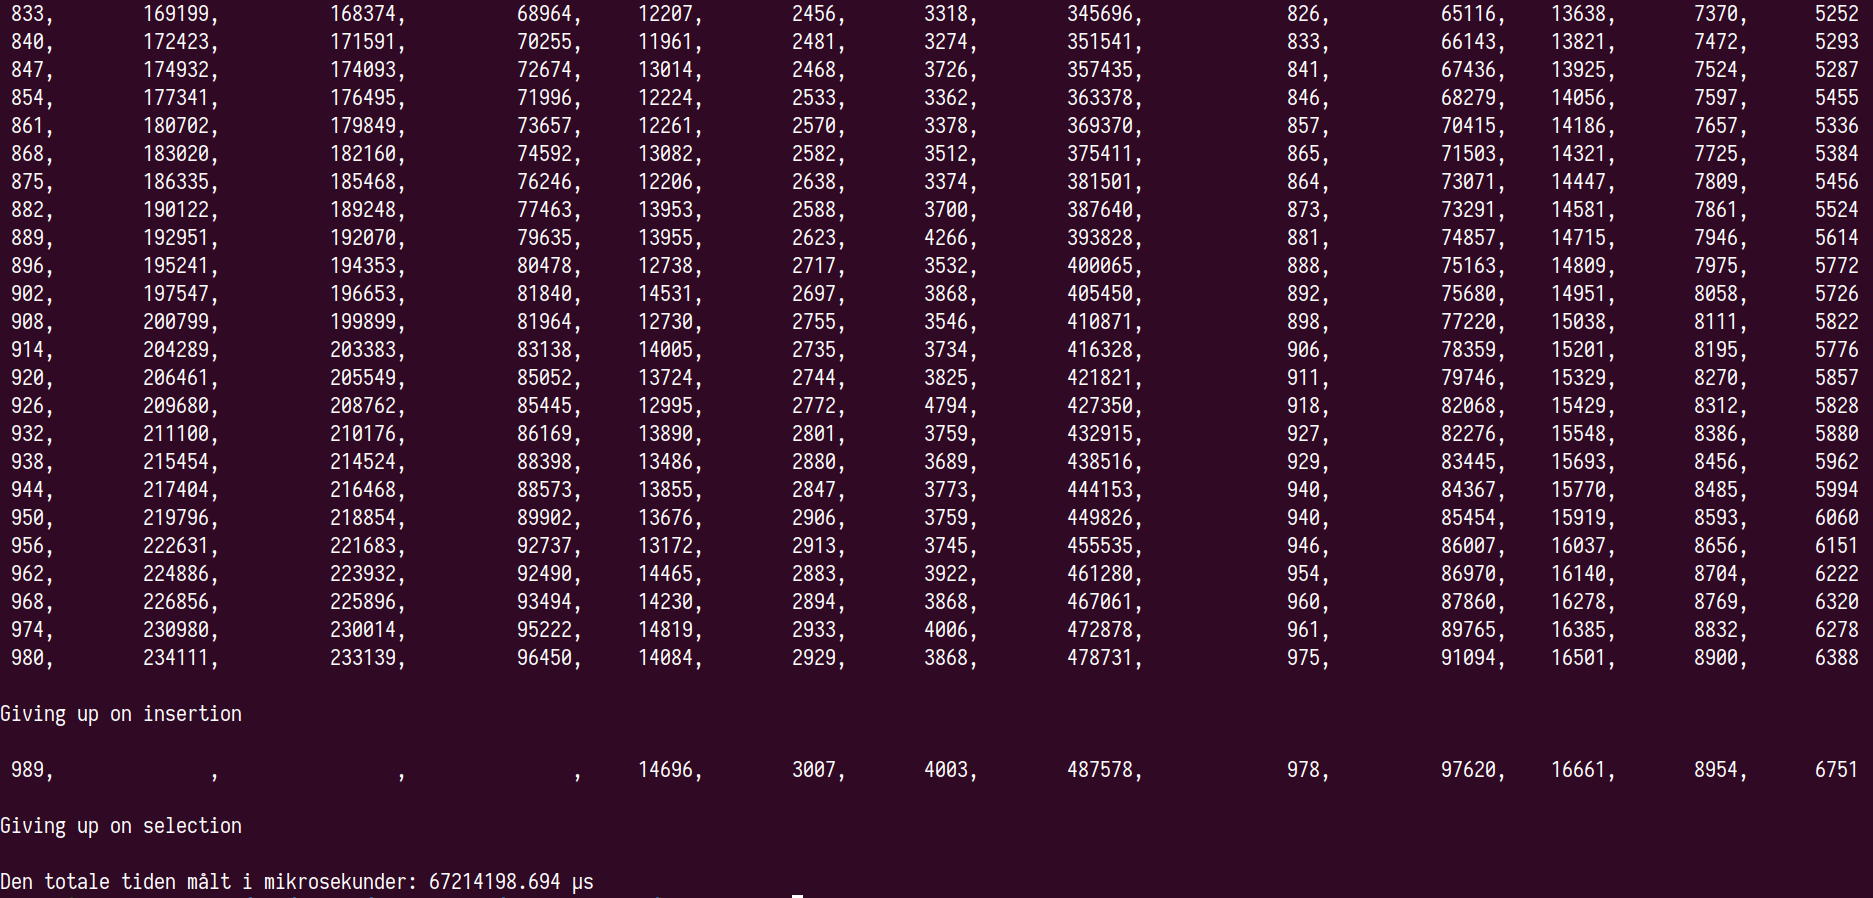
\includegraphics[scale=0.2]{IN2010oblig3_oppgave2d.png}
\\
Figur 6 - Outputen ved å kjøre filen 'random' med 1000 inputs.
\\
\subsection*{Deloppgave 3: Eksperimentér}
Nedenfor ser man ulike linjediagrammer som svarer til kjøretid for de ulike sorteringsalgoritmene hvor man ser hvordan antall inputs påvirker kjøretiden. Disse algoritmene er kjørt på både 'nearly sorted' og 'random' slik at man får et innblikk i når de ulike algoritmene er mest eller minst effektive. Dersom grafen som representerer en gitt sorteringsalgoritme plutselig stopper opp, så betyr det at kjøretiden for spesifikt et input bruker for lang tid i forhold til timelimiten som er oppgitt i prekoden. Da vil sorteringsalgoritmen breake, og vil dermed ikke fortsette å kjøre.
\\
\\
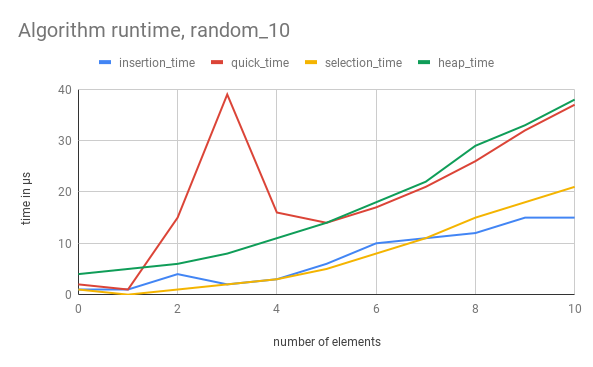
\includegraphics[scale=0.6]{Algorithm runtime, random_10.png}
\\
Figur 7 - Kjøretiden på de ulike sorteringsalgoritmene brukt på random-filen med 10 inputs.
\\
\\
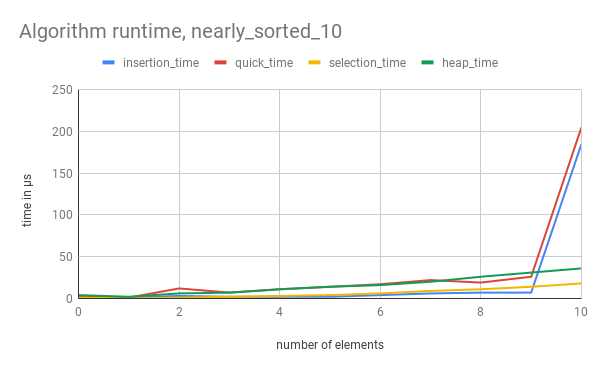
\includegraphics[scale=0.65]{Algorithm runtime, nearly_sorted_10.png}
\\
Figur 8 - Kjøretiden på de ulike sorteringsalgoritmene brukt på nearly-sorted-filen med 10 inputs.
\\
\\
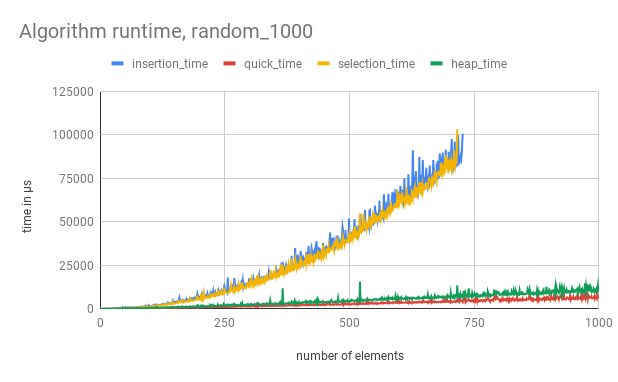
\includegraphics[scale=0.65]{Algorithm runtime.png}
\\
Figur 9 - Kjøretiden på de ulike sorteringsalgoritmene brukt på random-filen med 1000 inputs.
\\
\\
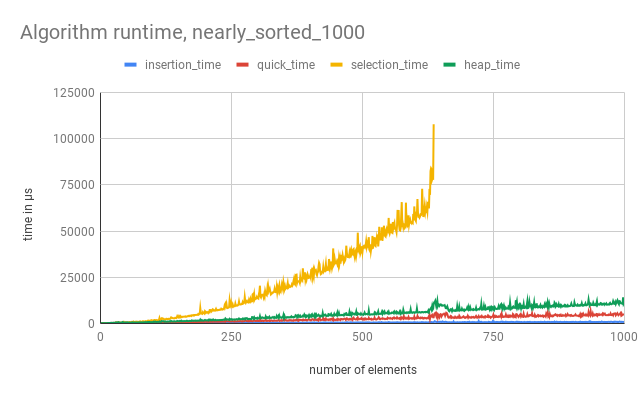
\includegraphics[scale=0.65]{Algorithm runtime_near.png}
\\
Figur 10 - Kjøretiden på de ulike sorteringsalgoritmene brukt på nearly-sorted-filen med 1000 inputs.
\\
\\
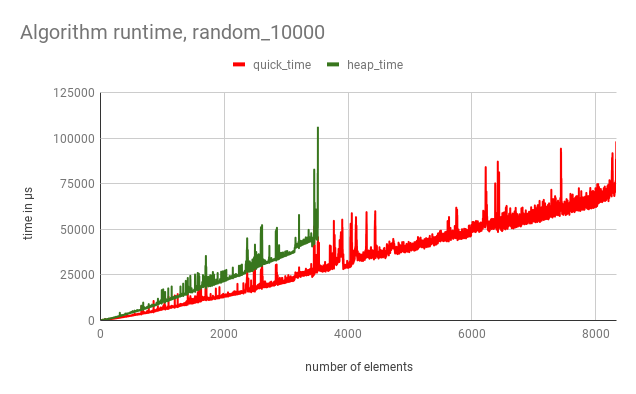
\includegraphics[scale=0.65]{Algorithm runtime, random_10000.png}
\\
Figur 11 - Kjøretiden på de ulike sorteringsalgoritmene brukt på random-filen med 10000 inputs.
\\
\\
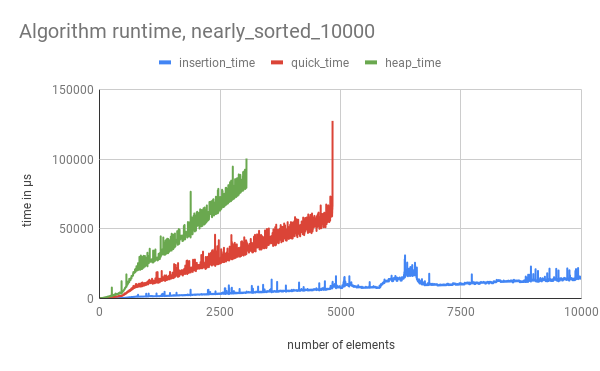
\includegraphics[scale=0.65]{Algorithm runtime, nearly_sorted_10000.png}
\\
Figur 12 - Kjøretiden på de ulike sorteringsalgoritmene brukt på nearly-sorted-filen med 10000 inputs.
\\
\\
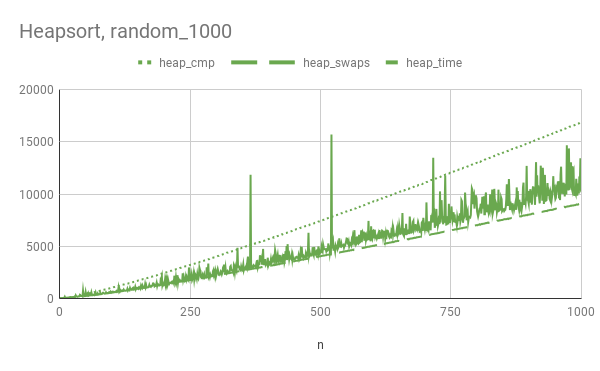
\includegraphics[scale=0.65]{Heapsort.png}
\\
Figur 13 - Antall sammenligninger, bytter og kjøretiden for heapsort brukt på random-filen med 1000 inputs.
\\
\\
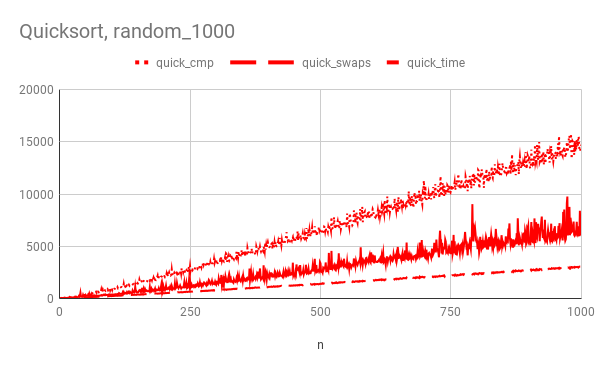
\includegraphics[scale=0.65]{Quicksort.png}
\\
Figur 14 - Antall sammenligninger, bytter og kjøretiden for quicksort brukt på random-filen med 1000 inputs.
\\
\\
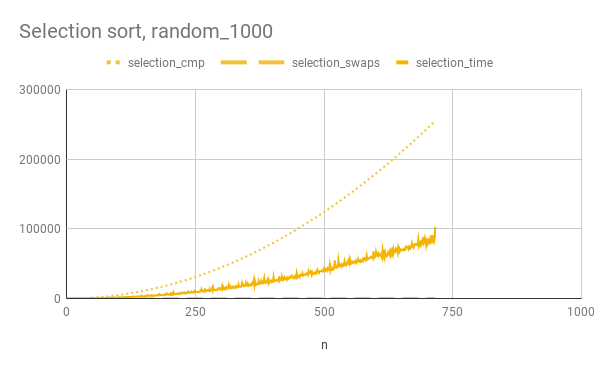
\includegraphics[scale=0.65]{Selection sort.png}
\\
Figur 15 - Antall sammenligninger, bytter og kjøretiden for selection sort brukt på random-filen med 1000 inputs.
\\
\\
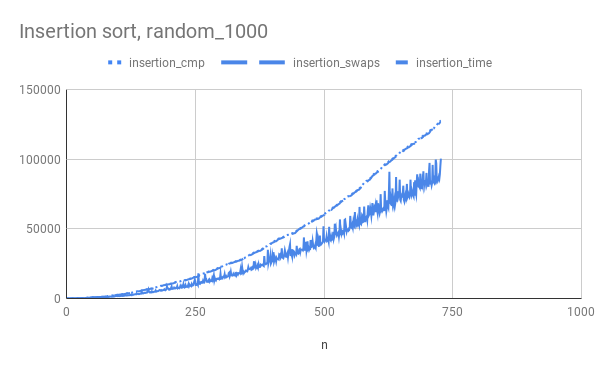
\includegraphics[scale=0.65]{Insertion sort.png}
\\
Figur 16 - Antall sammenligninger, bytter og kjøretiden for insertion sort brukt på random-filen med 1000 inputs.
\\
\\
\\
Hvilke sorteringsalgoritmer som utmerker seg positivt er avhengig av hva slags inputfil vi tester med. Dersom det er random-filen med 10 inputs, ser vi fra figur 7 at både insertion sort og selection sort gjør det best. Dersom det er nearly-sorted-filen med 10 inputs ser vi fra figur 8 at heapsort og selection sort gjør det best. Ved å se på disse to resultatene så vil det i gjennomsnitt være heapsort og selection sort som tar kortest tid.
\\
\\
På den andre siden kan vi se på hvilke sorteringsalgoritmer som er raskest dersom n er svært stor. Fra figur 9 observerer vi at for random-filen med relativt få inputs så har både insertion sort og selection sort svært høy kjøretid. Vi ser derfor bort fra disse sorteringalgoritmene for en stor n. Med samme argument ser man fra figur 10 at selection sort har lang kjøretid for nearly-sorted-filen. Dette fører oss til figur 11 og figur 12. Vi observerer her at quicksort er raskest for random-filen med 10000 inputs, ettersom heapsort bruker for lang tidd etter 3000 inputs og ender med å stoppe grunnet timelimiten vår. Derimot ser vi at insertion sort er raskest for nearly-sorted-filen med 10000 inputs. Denne er mye raskere enn de to andre, og klarer å bruke kort tid for hver input. I likhet med figur 11 ser vi at quicksort og heapsort også stopper etter x antall inputs. 
\\
\\
Dersom vi fokuserer på random-filen med 10000 inputs ser vi at quicksort og heapsort er relativt like med tanke på kjøretid. Den eneste store forskjellen er at heapsort blir avsluttet når n er litt over 3000. Siden både heapsort og quicksort har kjøretidskompleksitet $O(n \  log \ n)$ stemmer dette relativt bra med forventet resultat. På den andre siden stemmer ikke dette hvis vi ser på nearly-sorted-filen med 10000 inputs. Her har vi insertion sort som den raskeste som fullfører og er betraktelig raskere enn både quicksort og heapsort. Insertion sort har kjøretidskompleksitet $O(n^{2})$ mens de to andre har kjøretidskompleksitet $O(n \ log \ n)$. Dette er på grunn av at filen er nesten sortert fra før av, og følgende passer insertion svært godt for å løse det problemet. For å sammenligne kan vi referere til figur 9 som viser kjøretiden for alle sorteringsalgoritmene brukt på random-filen med 1000 inputs. Her ser vi at insertion sort og selection sort er omtrent like raske og at quicksort og heapsort er omtrent like raske. I tillegg er både heapsort og quicksort betydelig raskere enn de to andre sorteringsalgoritmene. Dette stemmer godt overens med kjøretidskompleksiteten på de ulike algoritmene.
\\
\\
ANTALL SAMMENLIGNINGER OG ANTALL BYTTER KORRELERT MED KJØRETIDkkk
\\
\end{document}